% https://pxl-digital.pxl.be/page/care-athon-2020#

De tweedaagse hackathon werd georganiseerd op de Corda Campus in gebouw 3 bij Cegeka. We werden hier ontvangen door Tristan Fransen en Francis Vos, die ons een korte introductie gaf over het onderwerp. Vervolgens maakten we kennis met de twee vertegenwoordigers van Ambulance Wens en Arno Barzan, de PXL\hyp{}begeleider van dit project. Arno Barzan gaf ons meer specifieke uitleg over wat er precies gerealiseerd moest worden en op welke manier. Mijn willekeurig ingedeelde team bestond uit vier studenten van applicatieontwikkeling en één systeem\hyp{} en netwerkbeheerder.

Ik heb gekozen voor de uitdaging van Ambulance Wens. Dit is een vzw die zich inzet voor mensen met een ongeneeslijke ziekte, die niet mobiel zijn en voelen dat hun heengaan nabij komt. Ze zorgen dat deze mensen hun laatste wens nog in vervulling kunnen brengen met de nodige medische ondersteuning. Zo kunnen ze een laatste keer met volle teugen genieten van het leven.

Omdat de interne organisatie en het tentoonstellen van wensen wat ouderwets was en stroef verliep, kregen wij de opdracht om een mobiele applicatie te ontwerpen voor de vzw. Aan de hand van deze app konden de pati"enten een wens kiezen en werd al het benodigd materiaal en personeel verzameld om te laten deelnemen aan deze wens. De nadruk lag dus vooral op de gebruiksvriendelijkheid en de consistentie van de applicatie.

Toen de hackathon daadwerkelijk van start ging, zijn we begonnen een taakverdeling in ons team, om de effici"entie van ons werk te vergroten. Zo focuste één student zich vooral op het maken van de mock\hyp{}ups, twee studenten op het onderzoek naar realiseerbaarheid en restricties van buitenaf en de overige twee studenten begonnen reeds met het ontwikkelen van de applicatie. Ik was één van die laatste twee, maar daarnaast hielp ik ook met het nemen van beslissingen in verband met de mock\hyp{}ups. De applicatie werd geschreven voor Android in Android Studio met Java als programmeertaal. De mock\hyp{}ups werden uitgewerkt in de webapplicatie van Marvel.

Rond het einde van de eerste dag zijn we als team tot het besluit gekomen dat we geen volledig uitgewerkte applicatie konden aanmaken in de voorziene tijd. Daarom zijn we gedurende de tweede dag ons meer gaan focussen op het afwerken en verfijnen van de mock\hyp{}ups, omdat we het idee naar voren brengen belangrijker vonden dan het afleveren van een half afgewerkt product. Op dat moment hebben we de taakverdeling opnieuw herschikt en zijn we dus met drie studenten aan de slag gegaan met de mock\hyp{}ups, terwijl de andere twee studenten verder onderzoek uitvoerden naar elementen als server hosting en GDPR\hyp{}wetgeving.

\begin{figure}[!h]
  \centering
  \begin{subfigure}[h]{0.3\textwidth}
    \centering
    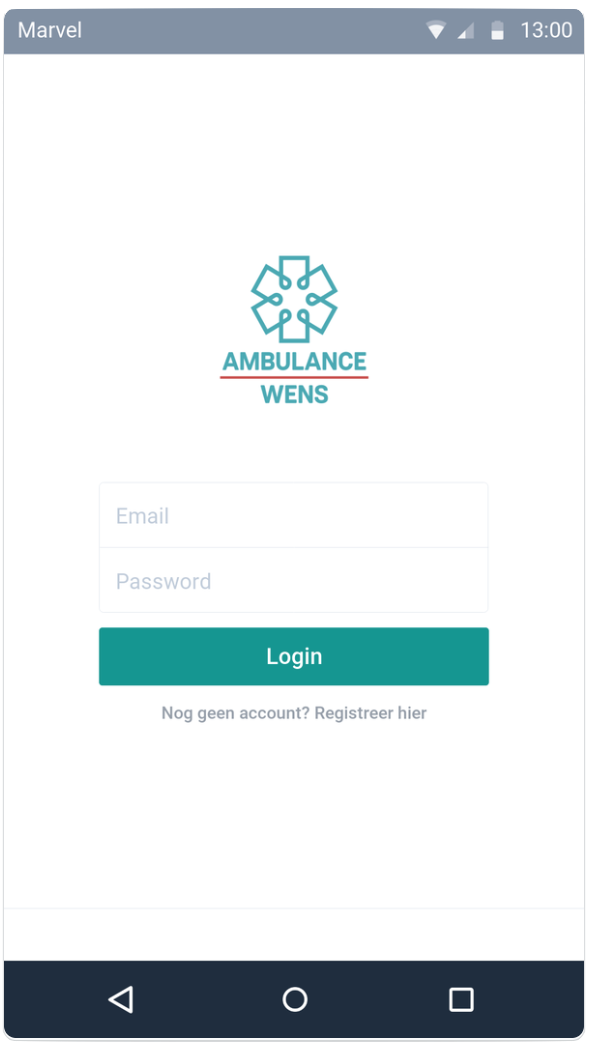
\includegraphics[width=0.76\textwidth]{images/care-athon/login.png}
  \end{subfigure}
  \begin{subfigure}[h]{0.3\textwidth}
    \centering
    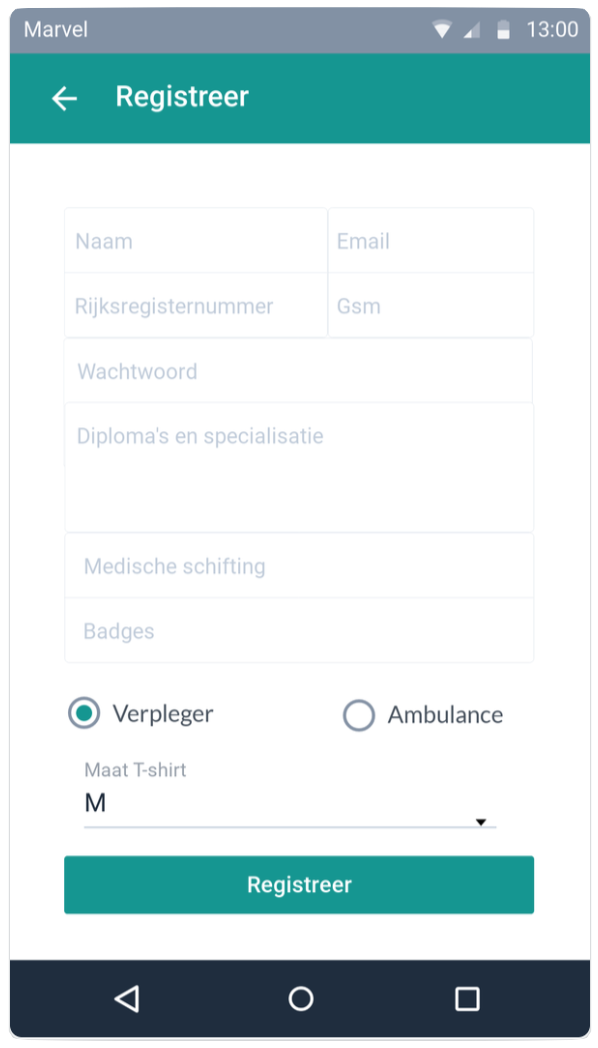
\includegraphics[width=0.76\textwidth]{images/care-athon/registreer.png}
  \end{subfigure}
  \begin{subfigure}[h]{0.3\textwidth}
    \centering
    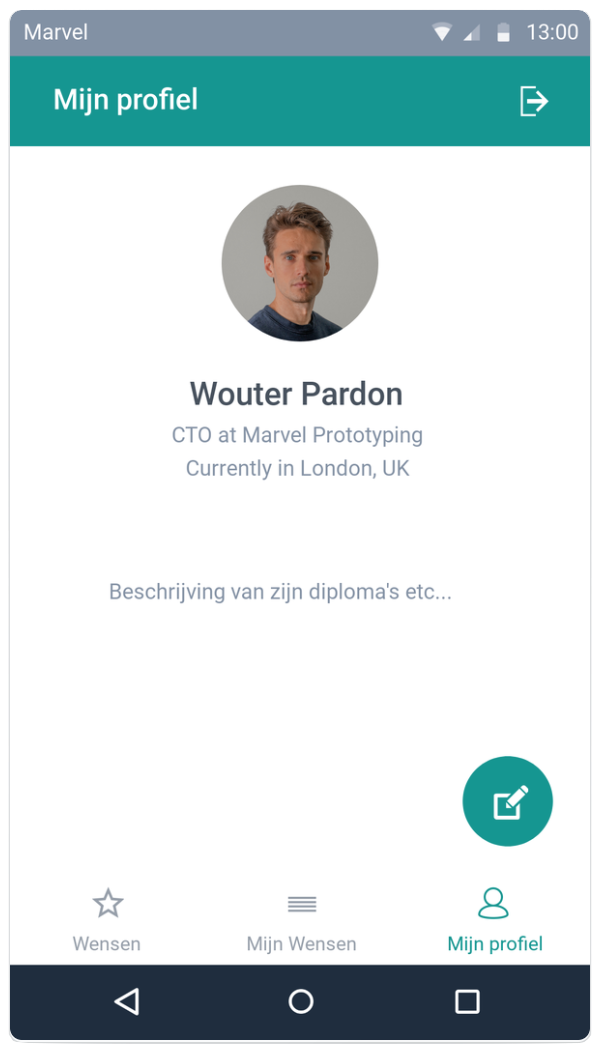
\includegraphics[width=0.76\textwidth]{images/care-athon/profiel.png}
  \end{subfigure}
\end{figure}

We konden op regelmatige basis feedback gaan vragen aan Arno Barzan en de twee vertegenwoordigers van Ambulance Wens, hetgeen ons meer inspiratie en duidelijkheid gaf over de opdracht, met een positief gevolg op onze applicatie. Zo wisten we welke informatie van de pati"enten, vrijwilligers en verplegers nodig was om de wens uit te kunnen voeren, en konden we het opvragen van deze info ook in onze applicatie verwerken. Anderzijds kregen we op die manier ook een beter idee over stijl waarin zij het liefst hun applicatie gezien hadden.

Op het einde van de hackaton presenteerde elke groep zijn applicatie voor de medestudenten, ook die van de andere uitdagingen. Onze presentatie was een demo van de applicatie aan de hand van de mock\hyp{}ups. Aangezien we ons onderzoek ook aan Ambulance Wens wilden overhandigen, hadden we een document gemaakt met alle gevonden informatie alsook onze mening over bepaalde beslissingen die gemaakt moesten worden.

Aan het einde van de hackathon kwam iedereen die hieraan deelnam samen in een aula om te luisteren naar verschillende sprekers. Daarop volgend waren de presentaties van alle teams. Na deze presentaties volgde de nominatie van de winnaars van elke uitdaging. Zij ontvingen een prijs afhankelijk van hun gekozen uitdaging.

Ik heb veel praktische zaken bijgeleerd van deze hackathon, zoals het maken van mock\hyp{}ups en het ontwikkelen van een applicatie met zeer specifieke restricties. Nooit voordien had ik zo een sterke nadruk gelegd op het maken van mock\hyp{}ups. Dit leerde ik van de student applicatieontwikkeling met full\hyp{}stack development als keuzetraject. Maar ook het feit dat we dermate moesten nadenken over het uitzicht van de applicatie in combinatie met de grote hoeveelheid eisen en restricties, heeft mijn visie over bepaalde aspecten van het ontwerp en de ontwikkeling zelf van projecten sterk be"invloed.

Daarnaast was de deelname aan een hackathon op zich ook nieuw voor mij. Het was een zeer verruimende ervaring, die mij op een zeer korte tijd in team veel nieuwe dingen over het uitwerken van een applicatie heeft bijgeleerd. Ik vind dat deze opdracht zeker een bijdrage heeft geleverd aan mijn opleiding en ik ben dus ook van mening dat dit in de opleiding vervat zou moeten blijven. Daarnaast heeft het mij ook doen inzien wat een software\hyp{}manager kan betekenen voor een team, omdat deze functie in ons team ontbrak en ik bijgevolg dit kon vergelijken met teams die er wel één of zelfs meerderen hadden. Zij konden veel meer structuur brengen in hun opdracht en gingen meer georganiseerd te werk in vergelijking met ons team.

Het luisteren naar de idee"en van de andere teams tijdens hun presentatie was eveneens leerzaam en amusant, aangezien je op die manier opnieuw met andere visies over bepaalde zaken in contact kwam, en ik op die manier weer mijn eigen visie kon verruimen. Omdat de organisatie voor een goed doel werkte, en niet enkel winstgevend voor het bedrijf, zette ik mij meer in voor de opdracht aangezien ik zelf ook deze mening deel met betrekking tot hun standpunten.

\begin{figure}[!h]
  \centering
  \begin{subfigure}[h]{0.3\textwidth}
    \centering
    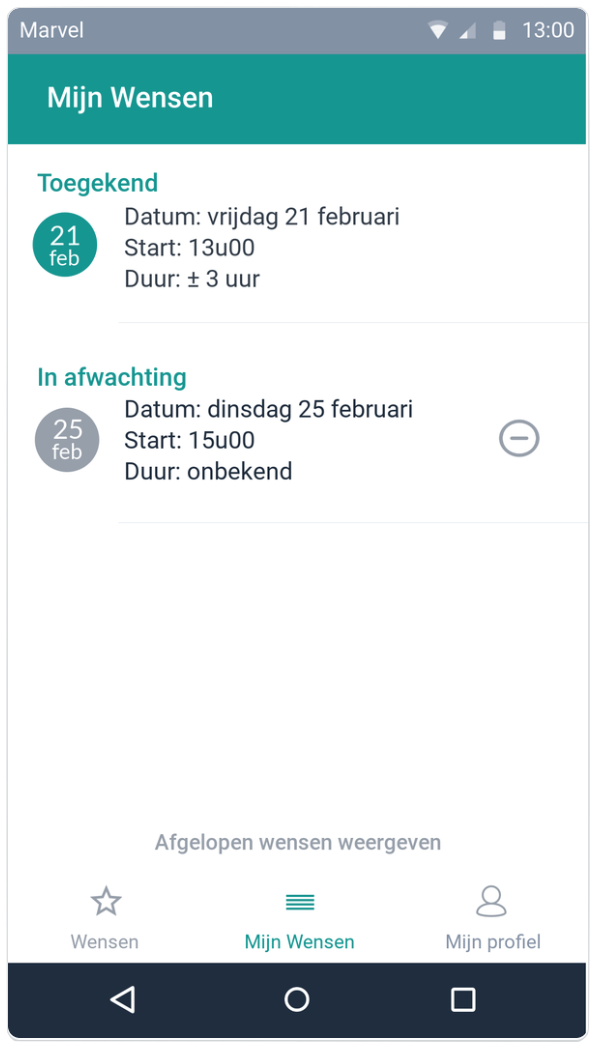
\includegraphics[width=0.685\textwidth]{images/care-athon/wensen.png}
  \end{subfigure}
  \begin{subfigure}[h]{0.3\textwidth}
    \centering
    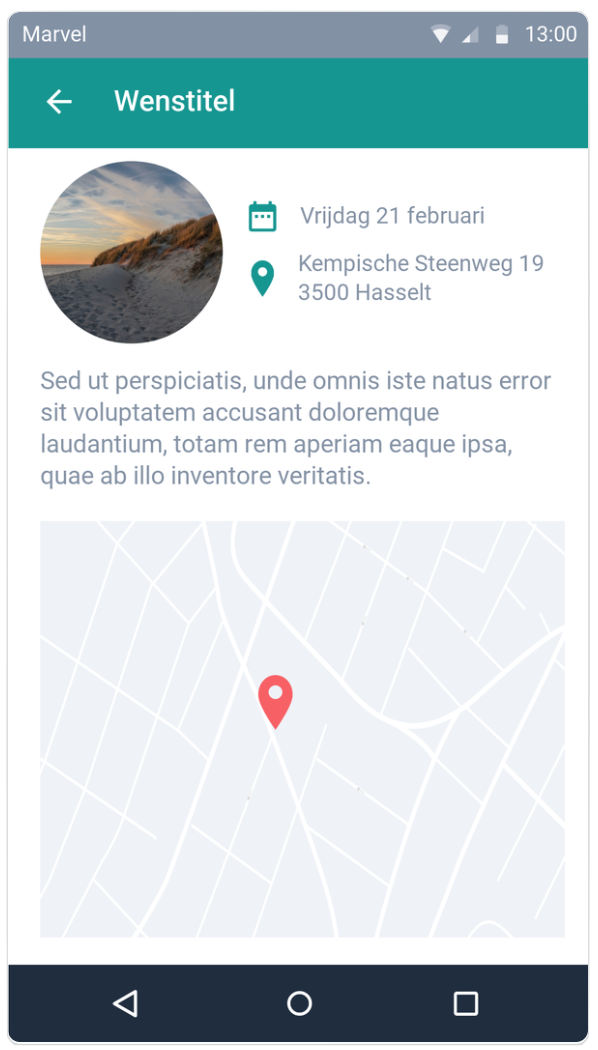
\includegraphics[width=0.685\textwidth]{images/care-athon/wens.png}
  \end{subfigure}
  \begin{subfigure}[h]{0.3\textwidth}
    \centering
    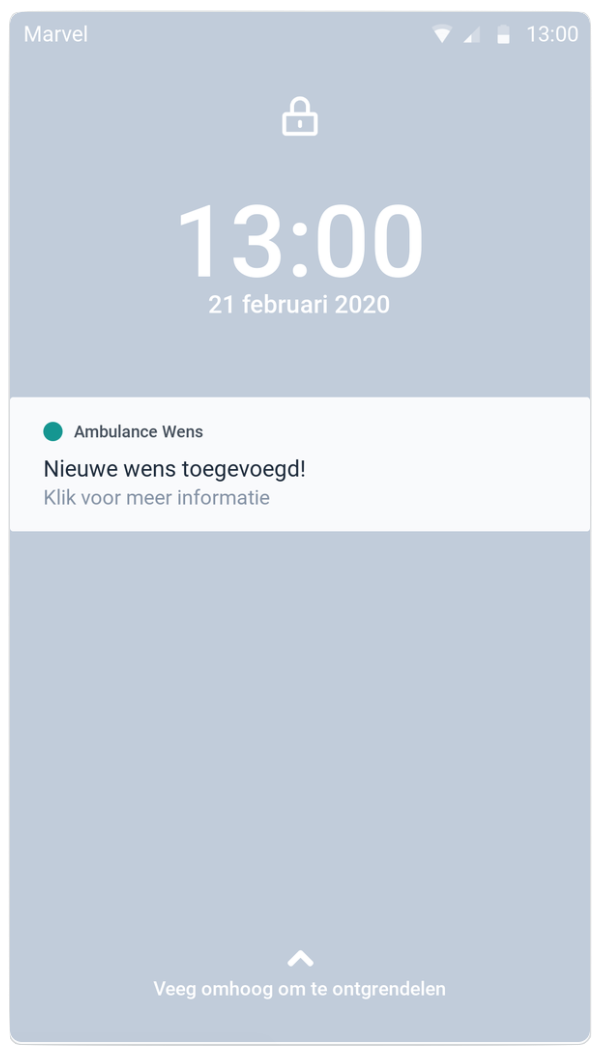
\includegraphics[width=0.685\textwidth]{images/care-athon/notificatie.png}
  \end{subfigure}
\end{figure}